\chapter{``Floats'' para Tabelas e Figuras}
Com os ambientes flutuantes, o \LaTeX\ oferece um mecanismo poderoso e conveniente para organizar figuras e tabelas automaticamente. Frequentemente, iniciantes não entendem corretamente esses ambientes flutuantes. Eles geralmente pedem para especificar a posição exata de uma tabela ou figura dentro do texto. No entanto, isso geralmente é desnecessário, pois o texto conterá referências a esses ambientes flutuantes. Também não é sensato porque tal objeto só pode ser definido na página se houver espaço suficiente para ele. Se esse não for o caso, o objeto teria que ser deslocado para a próxima página, possivelmente deixando um enorme espaço vazio na página anterior.

Frequentemente, um documento usará o mesmo argumento opcional para posicionar cada objeto flutuante. Isso também não faz sentido. Em tais casos, você deve alterar o valor padrão globalmente.

Uma nota final importante antes de começar esta seção: a maioria dos mecanismos descritos aqui, que estendem os recursos das classes padrão, não funcionam mais corretamente quando usados com pacotes que modificam a aparência das legendas de figuras e tabelas. Isso deveria ser evidente, mas é frequentemente esquecido.

\begin{figure}[h]
    \centering
    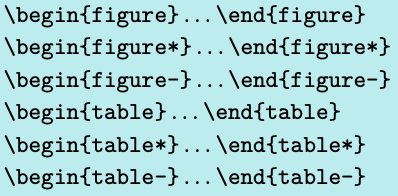
\includegraphics[width=0.5\linewidth]{imagem24.png}
\end{figure}